%\section{Distribution of IVOA Virtual Observatories Worlwide and its Projects}
\section{IVOA Virtual Observatories Worldwide}


\rem{MA}{Necessity of worldwideness}
\begin{itemize}
\item distributed astronomy facilities
\item unnecessary redundancy of observations and work
\end{itemize}

\rem{MA}{Data Deluge}

\rem{MA}{Why is difficult virtual centers worldwide}
\begin{itemize}
\item to organize the inherent diversity: different goals, working-style, budgets, language
\item why it can be done in science: public data, collaboration, etc
\end{itemize}


\subsection{The IVOA}
\rem{MA}{Check this section}

From June 2002, projects of virtual observatories have come to integrate the
International Virtual Observatory Alliance (IVOA) under the \textbf{Guidelines
for Participation\footnote{The guidelines are available in a paper in PDF and
DOC format from
\url{http://www.ivoa.net/documents/latest/IVOAParticipation.html}}}. These were
founded through national and international governmental and private programs in
collaboration with various centers of scientific studies, universities and
others. Who integrate this project, the Virtual Observatory (VO), share
knowledge between them and the community in a standardized manner. They
themselves are who develop these standards for data exchange and
interoperability. 




The table \ref{table:partners} shows the partners of IVOA to
November 2013.\\

\begin{table}%[h!t]
\centering
%\begin{tabular}{|p{7cm}|p{7cm}|}
\begin{tabular}{|l|l|}
	\hline
	\textbf{Project} & \textbf{URL} \\
	\hline
	NOVA (Argentina) & \url{http://nova.conicet.gov.ar/} \\
	\hline
	ARVO (Armenia) & \url{http://www.aras.am/Arvo/arvo.htm} \\
	\hline
	AstroGrid (United Kingdom) & \url{http://www.astrogrid.org/} \\
	\hline
	Aus-VO (Australia) & \url{http://aus-vo.org.au/} \\
	\hline
	BRAVO (Brazil) & \url{http://www.lna.br/bravo/} \\
	\hline
   CADC (Canada) &
    \url{http://www.cadc-ccda.hia-iha.nrc-cnrc.gc.ca} \\
	\hline
    ChiVO (Chile) & \url{http://www.chivo.cl/} \\
	\hline
    China-VO (China) &
    \url{http://www.china-vo.org/} \\
%	\hline
%    ESA-VO &
%    \url{http://www.sciops.esa.int/} \\
	\hline
	EURO-VO (Europe) & \url{http://www.euro-vo.org/} \\
	\hline
	GAVO (German) & \url{http://www.g-vo.org/} \\
	\hline
	HVO (Hungary) & \url{http://hvo.elte.hu/en/} \\
	\hline
	VObs.it (Italy) & \url{http://vobs.astro.it/} \\
	\hline
	JVO (Japan) & \url{http://jvo.nao.ac.jp/}\\
	\hline
	VO-France (France) & \url{http://www.france-vo.org/} \\
	\hline
	RVO (Russia) & \url{http://www.inasan.rssi.ru/eng/rvo/} \\
	\hline
	SVO (Spain) & \url{http://svo.cab.inta-csic.es/} \\
	\hline
	SA$^3$ (South Africa) & \url{http://www.sa3.ac.za/} \\
	\hline
	UkrVO (Ukrania) & \url{http://www.ukr-vo.org/} \\
	\hline
	VAO (United States) & \url{http://www.usvao.org/} \\
	\hline
	VOI (India) & \url{http://vo.iucaa.ernet.in/~voi/} \\
	\hline
\end{tabular}
\caption{IVOA's partners.}
\label{table:partners}
\end{table}

Almost half of IVOA virtual observatories are supported in Europe\footnote{The
Observatoire Virtuel France is ommited in \textbf{Europe} subsection of
\textbf{List of Virtual Observatories} section by lack of the information.} 9 of
the total; 1 belong to Africa, 1 to Australia, 2 to North America, 3 to South
America and 5 to Asia\footnote{As the mayor part of Rusia's territory is in
Asia, it will be considered like a virtual observatory of Asian continent.}. The
figure 1 shows the distribution of the IVOA's membership per continent.\\

%\begin{figure}%[h]
%\begin{center}
%	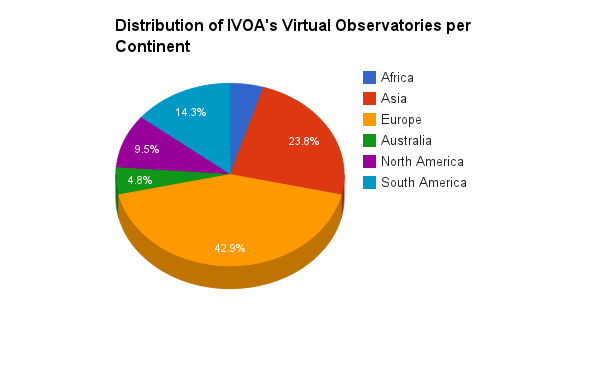
\includegraphics[scale=0.6]{img/vo_distribution.png}
%	\caption{International Virtual Observatory Alliance distribution per
%             continent.}
%\end{center}
%\end{figure}

\begin{figure}%[h]
\begin{center}
	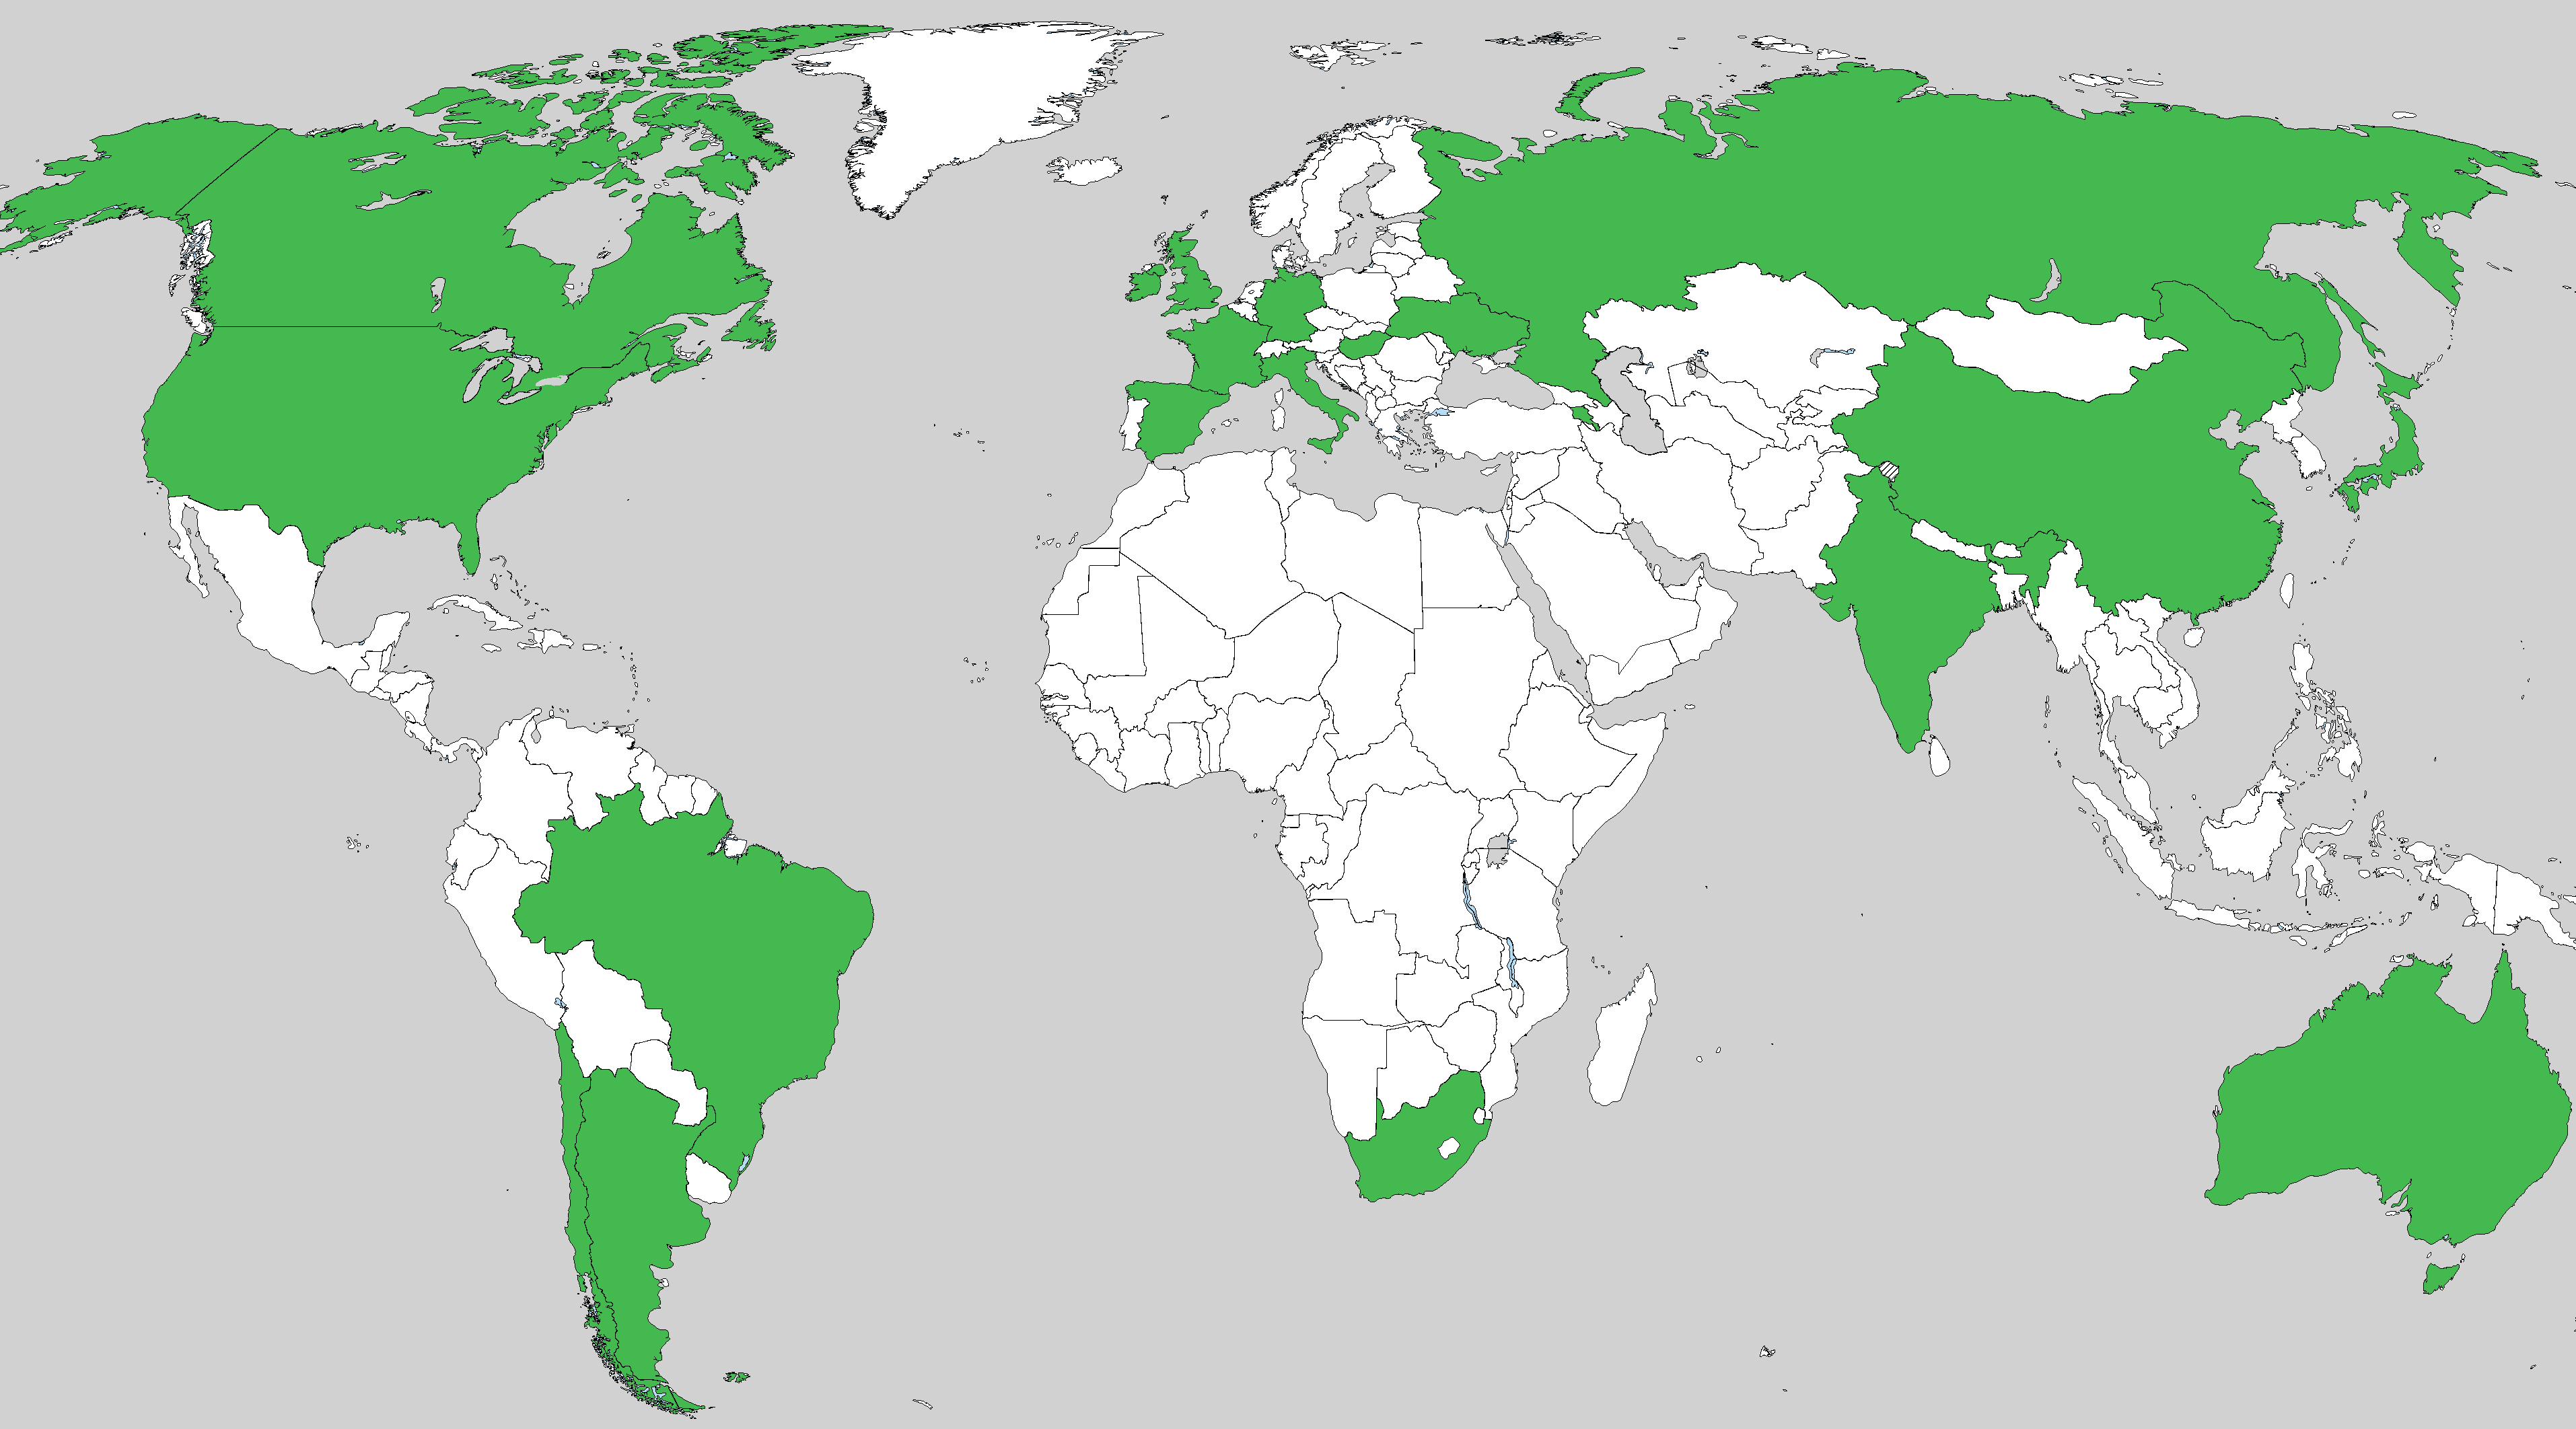
\includegraphics[width=0.9\linewidth]{img/VO-worldwide.png}
	\caption{International Virtual Observatory Alliance presence in the world.}
\end{center}
\end{figure}


\rem{JA}{A lot of initiatives converges in one and only VO. Access worldwide to 
scientists.}


\rem{MA}{subsec: Put here the infrastructure and the organizations}


\rem{MA}{Funding and Support: important actors of a VO}

\rem{MA}{subsec: Development lines of VOs and data speciality}

% If Chile became part of International Virtual Observatory Alliance, the
% distribution of IVOA's members per continent will be as shown in the figure
% 2. \\

%\begin{comment}
%\begin{figure}%[h]
%\begin{center}
%	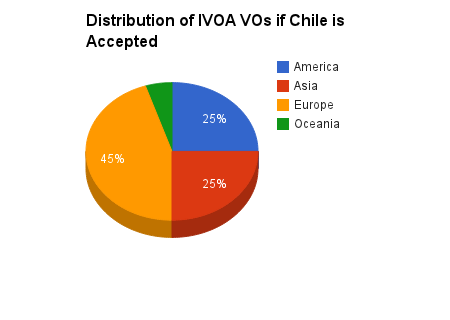
\includegraphics[width=110mm]{img/if_chile.png}
%	\caption{International Virtual Observatory Alliance distribution per
%             continent if Chile is accepted.}
%\end{center}
%\end{figure}
%\end{comment}

%Without considering the status of the internal projects of the virtual
%observatories, the membership of Chile would contribute to the cooperation,
%development and interoperability from America in the same percent that Asia.
%Furthermore, this fact would be very significant, because a large numbers of
%astronomical centers like observatories are placed in this country.  For now, is
%intended to work with a certain quantity of data of ALMA.\\



